%!TEX root = ../physical-olympics-2.tex
\chapter{光的衍射}


\section{光栅与波带片}
\begin{itemize}
\item 光栅衍射:\,光栅常数,\,即空间周期为$d$,\,缝宽为$a$,\,总共刻$N$道.\,那么:
\[I=I_0\cdot f_1(\theta)\cdot \left(\frac{\sin N\beta}{\sin \beta}\right)^2\quad, \quad \beta=\frac{\pi d}{\lambda}\sin \theta\]

其中$f_1(\theta)$为之后可以算出来的与单缝衍射有关的慢变(需要$a<<d$)的单元因子:
\[f_1(\theta)=\left(\frac{\sin \alpha}{ \alpha}\right)^2\quad, \quad \alpha=\frac{\pi a}{\lambda}\sin \theta\]

体现光栅的结构的是后面的结构因子:
\[f_2(\theta)=\left(\frac{\sin N\beta}{\sin \beta}\right)^2\quad, \quad \beta=\frac{\pi d}{\lambda}\sin \theta\]

从中可以得到三个信息:\,主极大方向$d\sin\theta_j=j\lambda$,\,主极大强度$I=N^2 I_0$,\,主极大宽度$\delta\theta\sim j\lambda/Nd$

\item 圆孔菲涅尔衍射:\,波带法与半波带法.\,核心在于以下等式:
\[\frac{\ud S}{r}={\rm const.}\cdot \ud r\]

\begin{figure}[H]
\centering
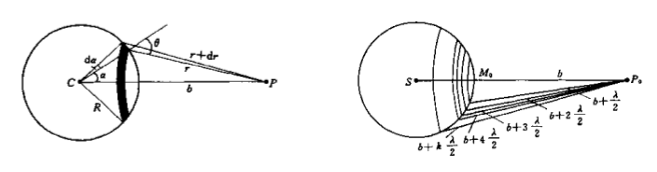
\includegraphics[width=0.8\textwidth]{image/14-2-2.png}
\caption{波带法与半波带法}
\end{figure}

这说明不同位置的波前上的带状面元,\,根据其对要计算的点所造成的光程差,\,相等的光程差造成完全相等的振幅,\,尽管面元的面积不相等.\,只需要把这些振幅相等,\,相位不等的光矢量进行合成.

合成方法一般有两种,\,对于半波带问题把面元分解为半波带显得方便.\,而复杂问题需要按照微元分解,\,下一节将介绍面元对要计算的点的光矢量贡献还有一个起到调制作用的角度因子,\,故合成图像一般为:
\begin{figure}[H]
\centering
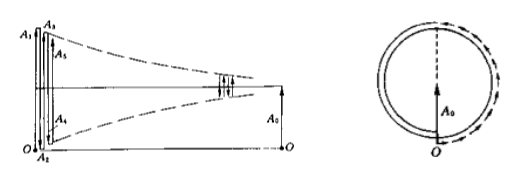
\includegraphics[width=0.8\textwidth]{image/14-2-3.png}
\caption{分组合成与积分合成}
\end{figure}

\item 波带片:\,预想将一点光源和一要计算光强的点中间合适距离处的波前按照半波带分解,\,再制造一光学器件,\,或者遮住奇数半波带而开放偶数半波带,\,或者遮住偶数半波带而开放奇数半波带.\,就构成了波带片.\,如果在一张圆形的片上入射平行光,\,而选取距离为$f$的点计算光程,\,那么各个半径为:
\[\rho_j=\sqrt{j\lambda f}\]

这样的波带片可以当做一个焦距为$f$的透镜使用.\,但是成像并不唯一,\,容易证明它具有一组虚焦点和实焦点.


\end{itemize}

%\section{布拉格衍射}

\section{衍射积分公式}

\begin{itemize}
\item 基尔霍夫衍射积分公式:
\[A(\bs{r})=\frac{1}{i\lambda}\int \bs{A}(\bs{r}')\cdot F\cdot \frac{e^{\ui k|\bs{r}-\bs{r}'|}\ud S}{|\bs{r}-\bs{r}'|}\]

$F$为角度因子,\,若入射波波矢$\bs{k}'$方向为$\bs{e}'$,\,子波波矢$\bs{k}$方向为$\bs{e}$,\,面元$\ud S$方向为$\bs{n}$,\,则有:
\[F=\frac{\bs{n}\cdot \bs{e}+\bs{n}\cdot \bs{e}'}{2}=\frac{\cos\theta+\cos \theta'}{2}\]

\item 夫琅和费衍射公式:\,如果在衍射屏后放置焦距为$f$的透镜并在后焦面上观察,\,并且忽略角度因子.\,把入射场在衍射屏作用后的波前写作$A(x_0,\,y_0)$.\,那么这个情况具有更简单的公式:
\[A(\theta_x,\,\theta_y)=\frac{1}{\ui\lambda f}\iint A(x_0,\,y_0)e^{-i(k_x x_0+k_y y_0)}\ud x_0\ud y_0\]

\item 矩孔衍射:
\[I=I_0\cdot \left(\frac{ab}{\lambda f}\right)^2\cdot \left(\frac{\sin\alpha}{\alpha}\right)^2\cdot \left(\frac{\sin\beta}{\beta}\right)^2\quad ,\quad \alpha =\frac{\pi a}{\lambda}\sin\theta_x\,,\,\beta =\frac{\pi b}{\lambda}\sin\theta_y\]

\item 圆孔衍射:\,直径$d$,\,艾里斑半角$\theta$:
\[\theta\approx \frac{1.22\lambda 	}{d}\]
\end{itemize}

%\section{波前分析法}
